\section{Placa Mãe}\label{sec:placa_mae}

A placa-mãe (Figura~\ref{fig:modulo_placa_mae}) é responsável por fazer a ligação entre os atuadores do robô, transmitindo potência da bateria para os módulos de motor e de chute, fazendo a ligação entre esses módulos e os respectivos atuadores, fornecendo tensão aos circuitos lógicos e fazendo a ligação entre o módulo de controle e os sensores do robô -, no caso um sensor de quadratura em cada motor e o sensor ótico do chute que verifica a posse da bola. 

\begin{figure}
	\centering
	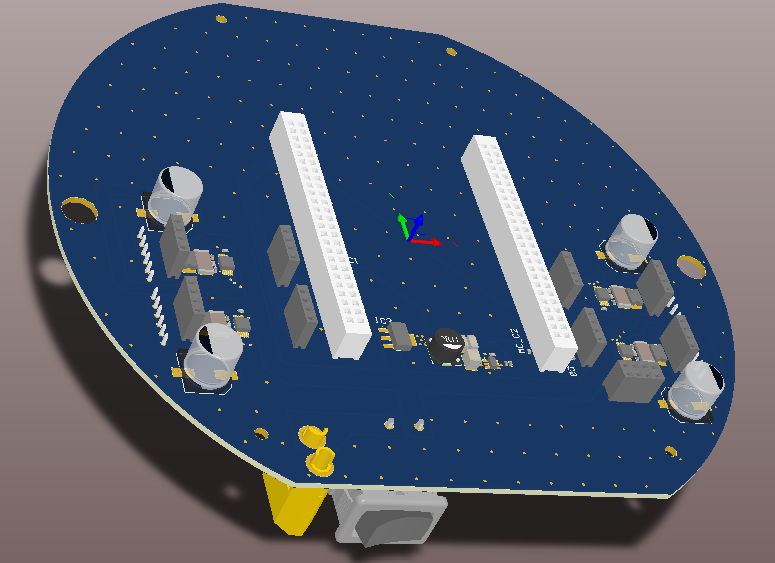
\includegraphics[scale=0.8]{modulo_placa_mae}
	\caption{Módulo da placa-mãe}
	\label{fig:modulo_placa_mae}
\end{figure}

\begin{figure}
	\centering
	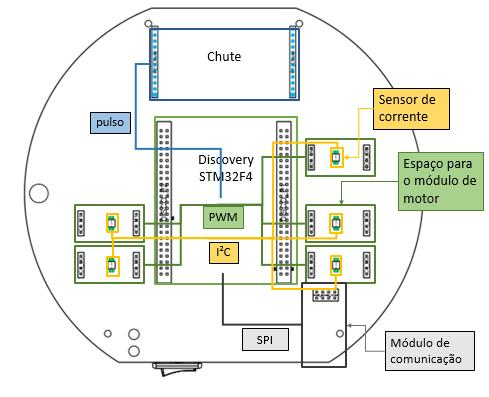
\includegraphics[scale=1]{blocos_placa_mae}
	\caption{Diagrama de blocos da placa mãe}
	\label{fig:blocos_placa_mae}
\end{figure}

Para que as conexões elétricas através da placa sejam feitas de modo seguro, a placa mãe contém um fusível, um capacitor de tanque, um capacitor de desacoplamento, e um sensor de corrente, o chip INA220, na entrada de cada módulo de motor e na entrada do módulo de chute, além de um circuito de divisão de tensão para que o módulo de controle seja capaz de controlar o nível de tensão da bateria.
O controle dessa placa é feito no \textit{firmware} através da classe INA220, que faz a comunicação com os sensores de corrente na placa e a classe bateria que controla o nível da bateria sendo usada pelo robô. Essas classes permitem o controle dos circuitos de segurança do robô de maneira que o \textit{firmware} possa lidar com comportamentos anômalos.
O desenho dessa placa foi reformulado:

\begin{itemize}
  \item As trilhas nos caminhos de potência foram trocados por planos para diminuir a resistência e o aquecimento das trilhas;
  \item Os antigos fusíveis simples foram trocados por fusíveis resetáveis para evitar que precisasse ser trocado durante a competição ou a 		cada sobrecorrente;
  \item Os antigos capacitores de tanque through hole foram trocados por capacitores SMD visando automatizar o processo de montagem utilizando 			uma pick and place automática;
  \item Os sensores de corrente também foram trocados por sua versão mais moderna e foi corrigido um erro no esquemático da placa mãe;
  \item O conector do módulo de transmissão foi trocado para ser compatível com o novo módulo de transmissão adotado pelo time.
\end{itemize}

% vim: tw=80 et ts=2 sw=2 sts=2 ft=tex spelllang=pt_br,en
